\documentclass{beamer}
\usepackage{beamerthemesplit}
\usepackage{wrapfig}
\usetheme{SPbGU}
\usepackage{pdfpages}
\usepackage{amsmath}
\usepackage{cmap} 
\usepackage[T2A]{fontenc} 
\usepackage[utf8]{inputenc}
\usepackage[english,russian]{babel}
\usepackage{indentfirst}
\usepackage{amsmath}
\usepackage{tikz}
\usepackage{multirow}
\usepackage[noend]{algpseudocode}
\usepackage{algorithm}
\usepackage{algorithmicx}
\usetikzlibrary{shapes,arrows}
%usepackage{fancyvrb}
%\usepackage{minted}
%\usepackage{verbments}


\title[]{YaccConstructor}
\subtitle[YaccConstructor]{Задачи на осенний семестр 2017}
% То, что в квадратных скобках, отображается в левом нижнем углу. 
\institute[]{
Лаборатория языковых инструментов JetBrains \\
Санкт-Петербургский государственный университет \\
Математико-механический факультет }

% То, что в квадратных скобках, отображается в левом нижнем углу.
\author[Семён Григорьев]{Семён Григорьев}

\date{8 сентября 2017г.}

\definecolor{orange}{RGB}{179,36,31}

\begin{document}
{
\begin{frame}[fragile]
  \begin{tabular}{p{2.5cm} p{5.5cm} p{2cm}}
   \begin{center}
      
\includegraphics[height=1.5cm]{pictures/JBLogo3.pdf}
    \end{center}
    &
    \begin{center}
      
\includegraphics[height=1.5cm]{pictures/SPbGU_Logo.png}
    \end{center}
    &
    \begin{center}
      
\includegraphics[height=1.5cm]{pictures/YC_logo.pdf}
    \end{center} 
  \end{tabular}
  \titlepage
\end{frame}
}

\begin{frame}[fragile]
  \transwipe[direction=90]
  \frametitle{YaccConstructor}
  \begin{itemize}
    \item Исследования в области формальных языков
    \item Открытый исходный код
    \begin{itemize}
      \item \url{https://github.com/YaccConstructor}
    \end{itemize}
    \item Основной язык разработки --- F\#
  \end{itemize}
\end{frame}

\begin{frame}[plain,c]
 \transwipe[direction=90]
 \begin{center}
  \Huge Применение методов ``машинного обучения'' к классификации цепочек (16s) на основе их вторичной структуры
 \end{center}
\end{frame}

\begin{frame}[fragile]
\transwipe[direction=90]
\frametitle{Вторичная структура}
  
   \begin{center}
      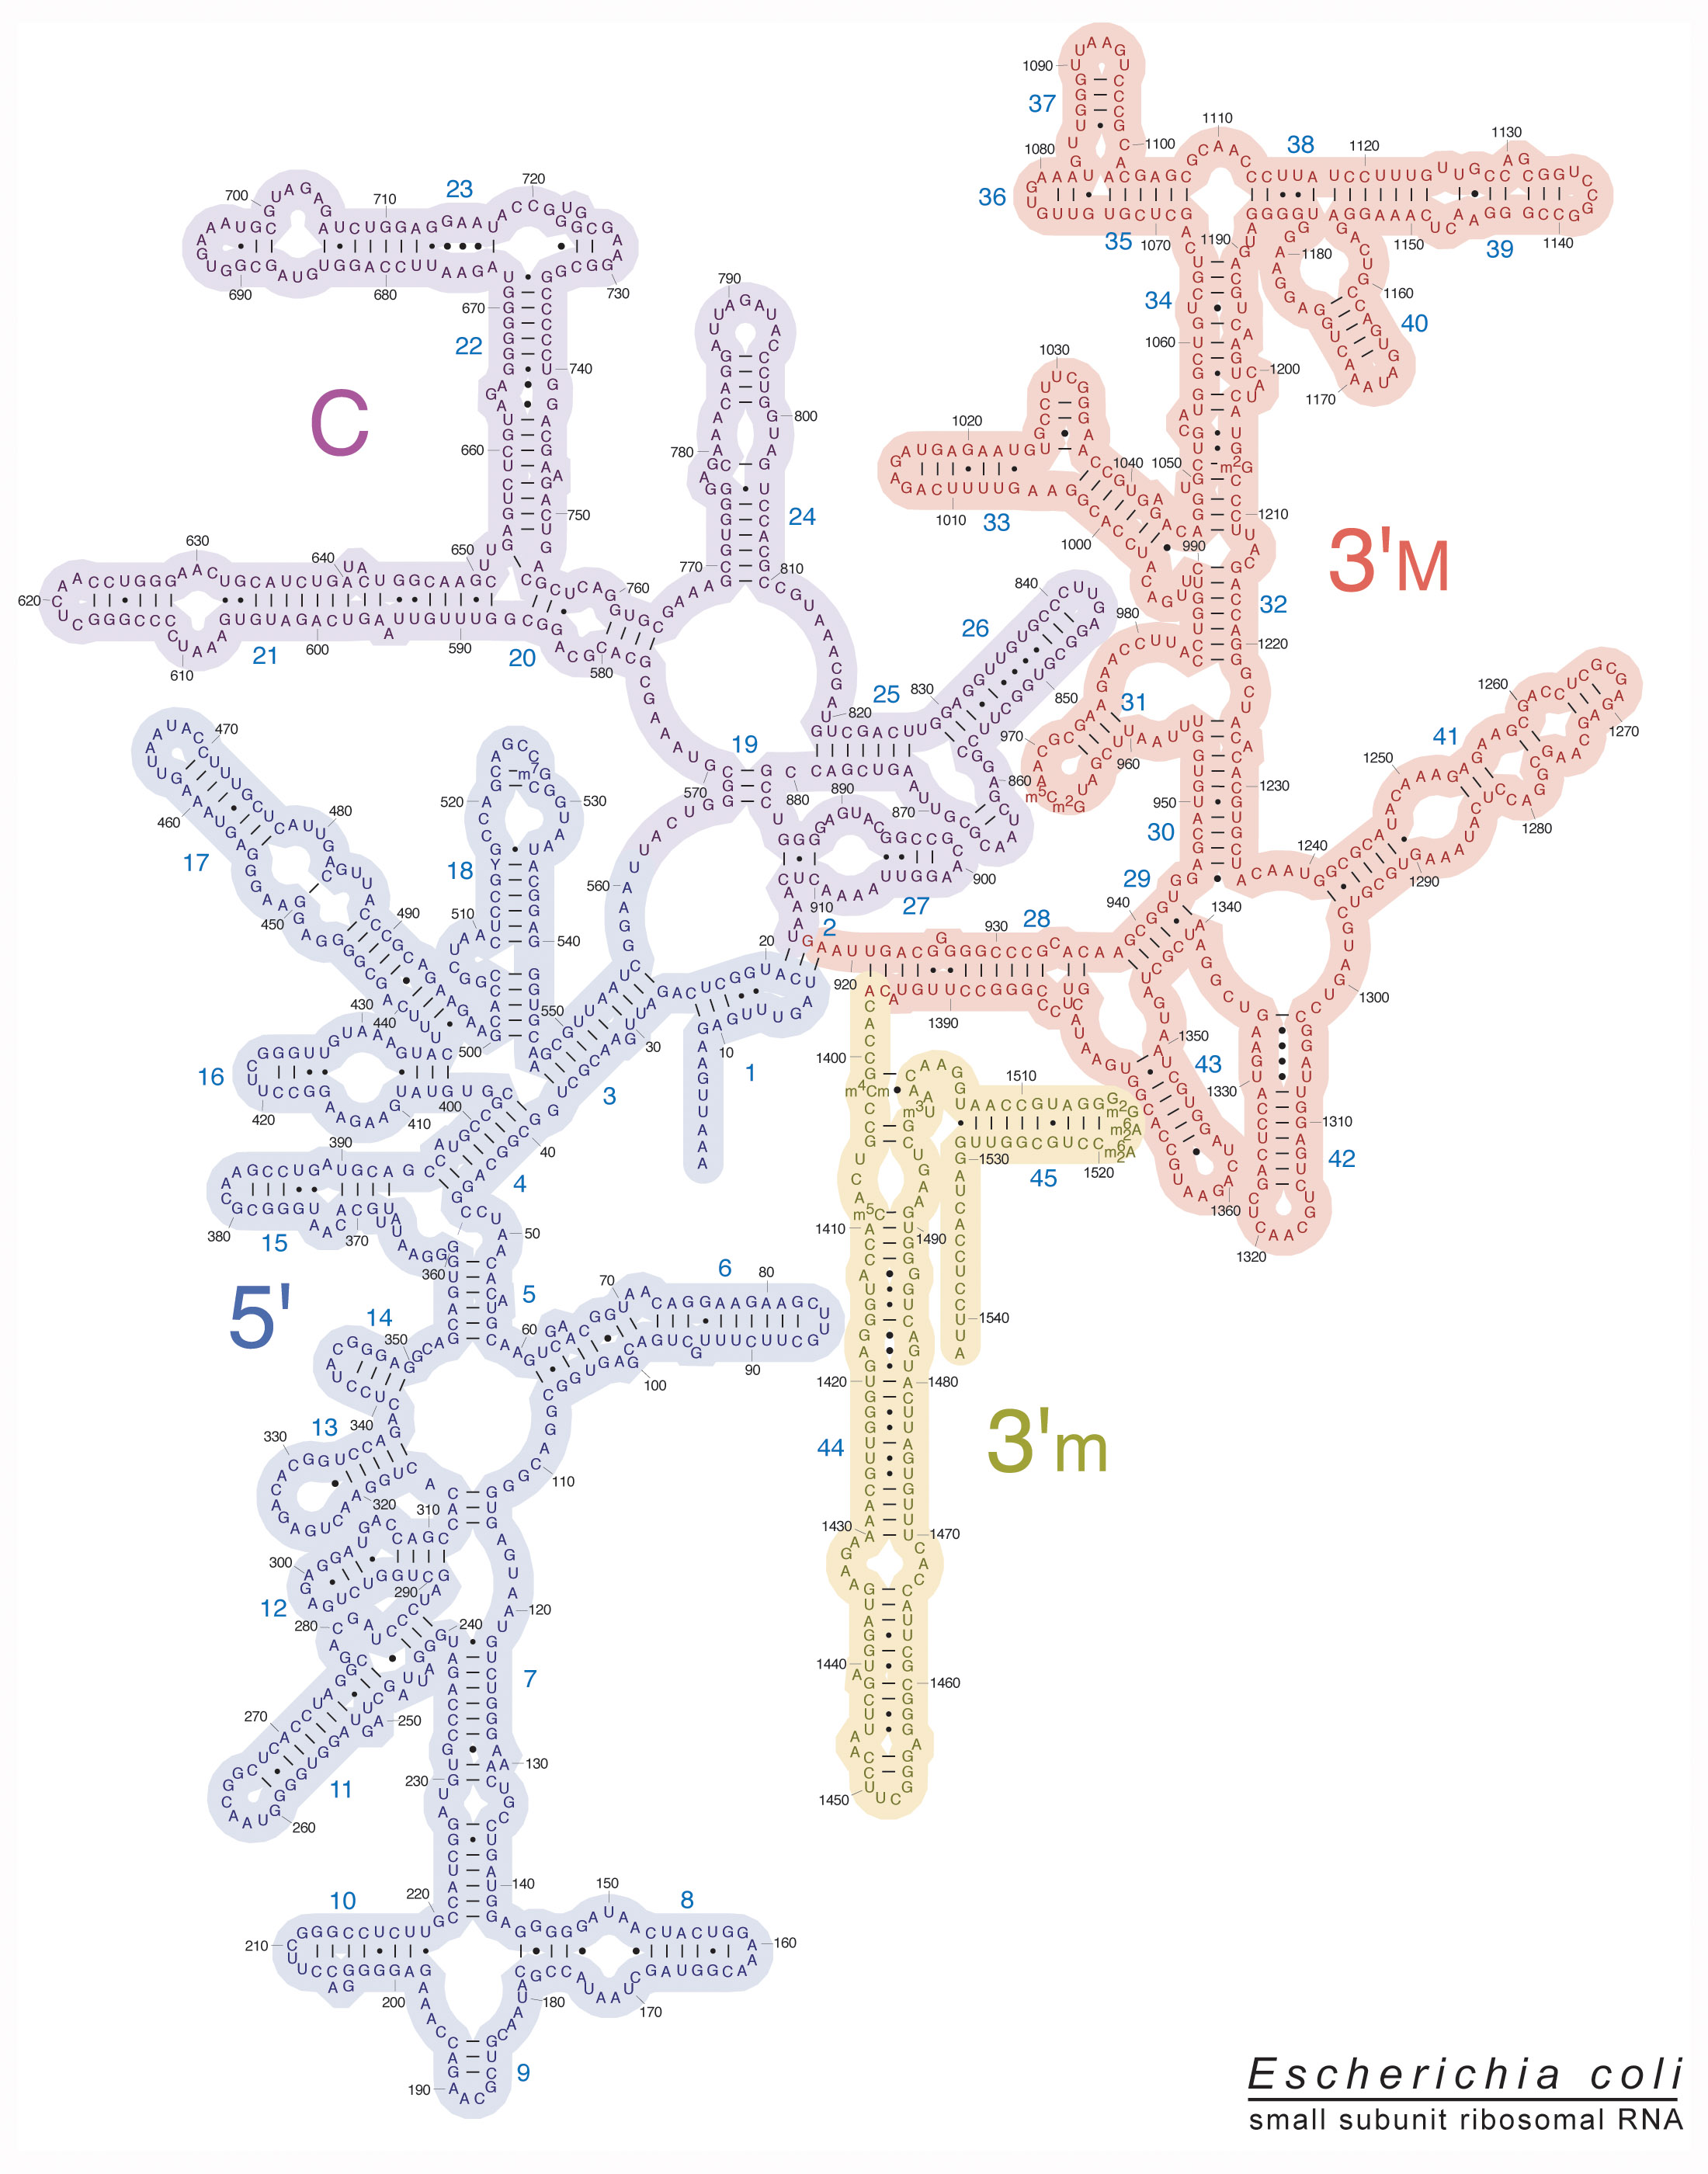
\includegraphics[height=8cm]{pictures/ecoli_16s.jpg}
    \end{center}
  
\end{frame}


\begin{frame}[fragile]
\transwipe[direction=90]
\frametitle{Примеры изображений}
  \begin{tabular}{p{6cm} p{6cm}}
   \begin{center}
      
\includegraphics[height=5.4cm]{pictures/bw.png}
    \end{center}
    &
    \begin{center}
      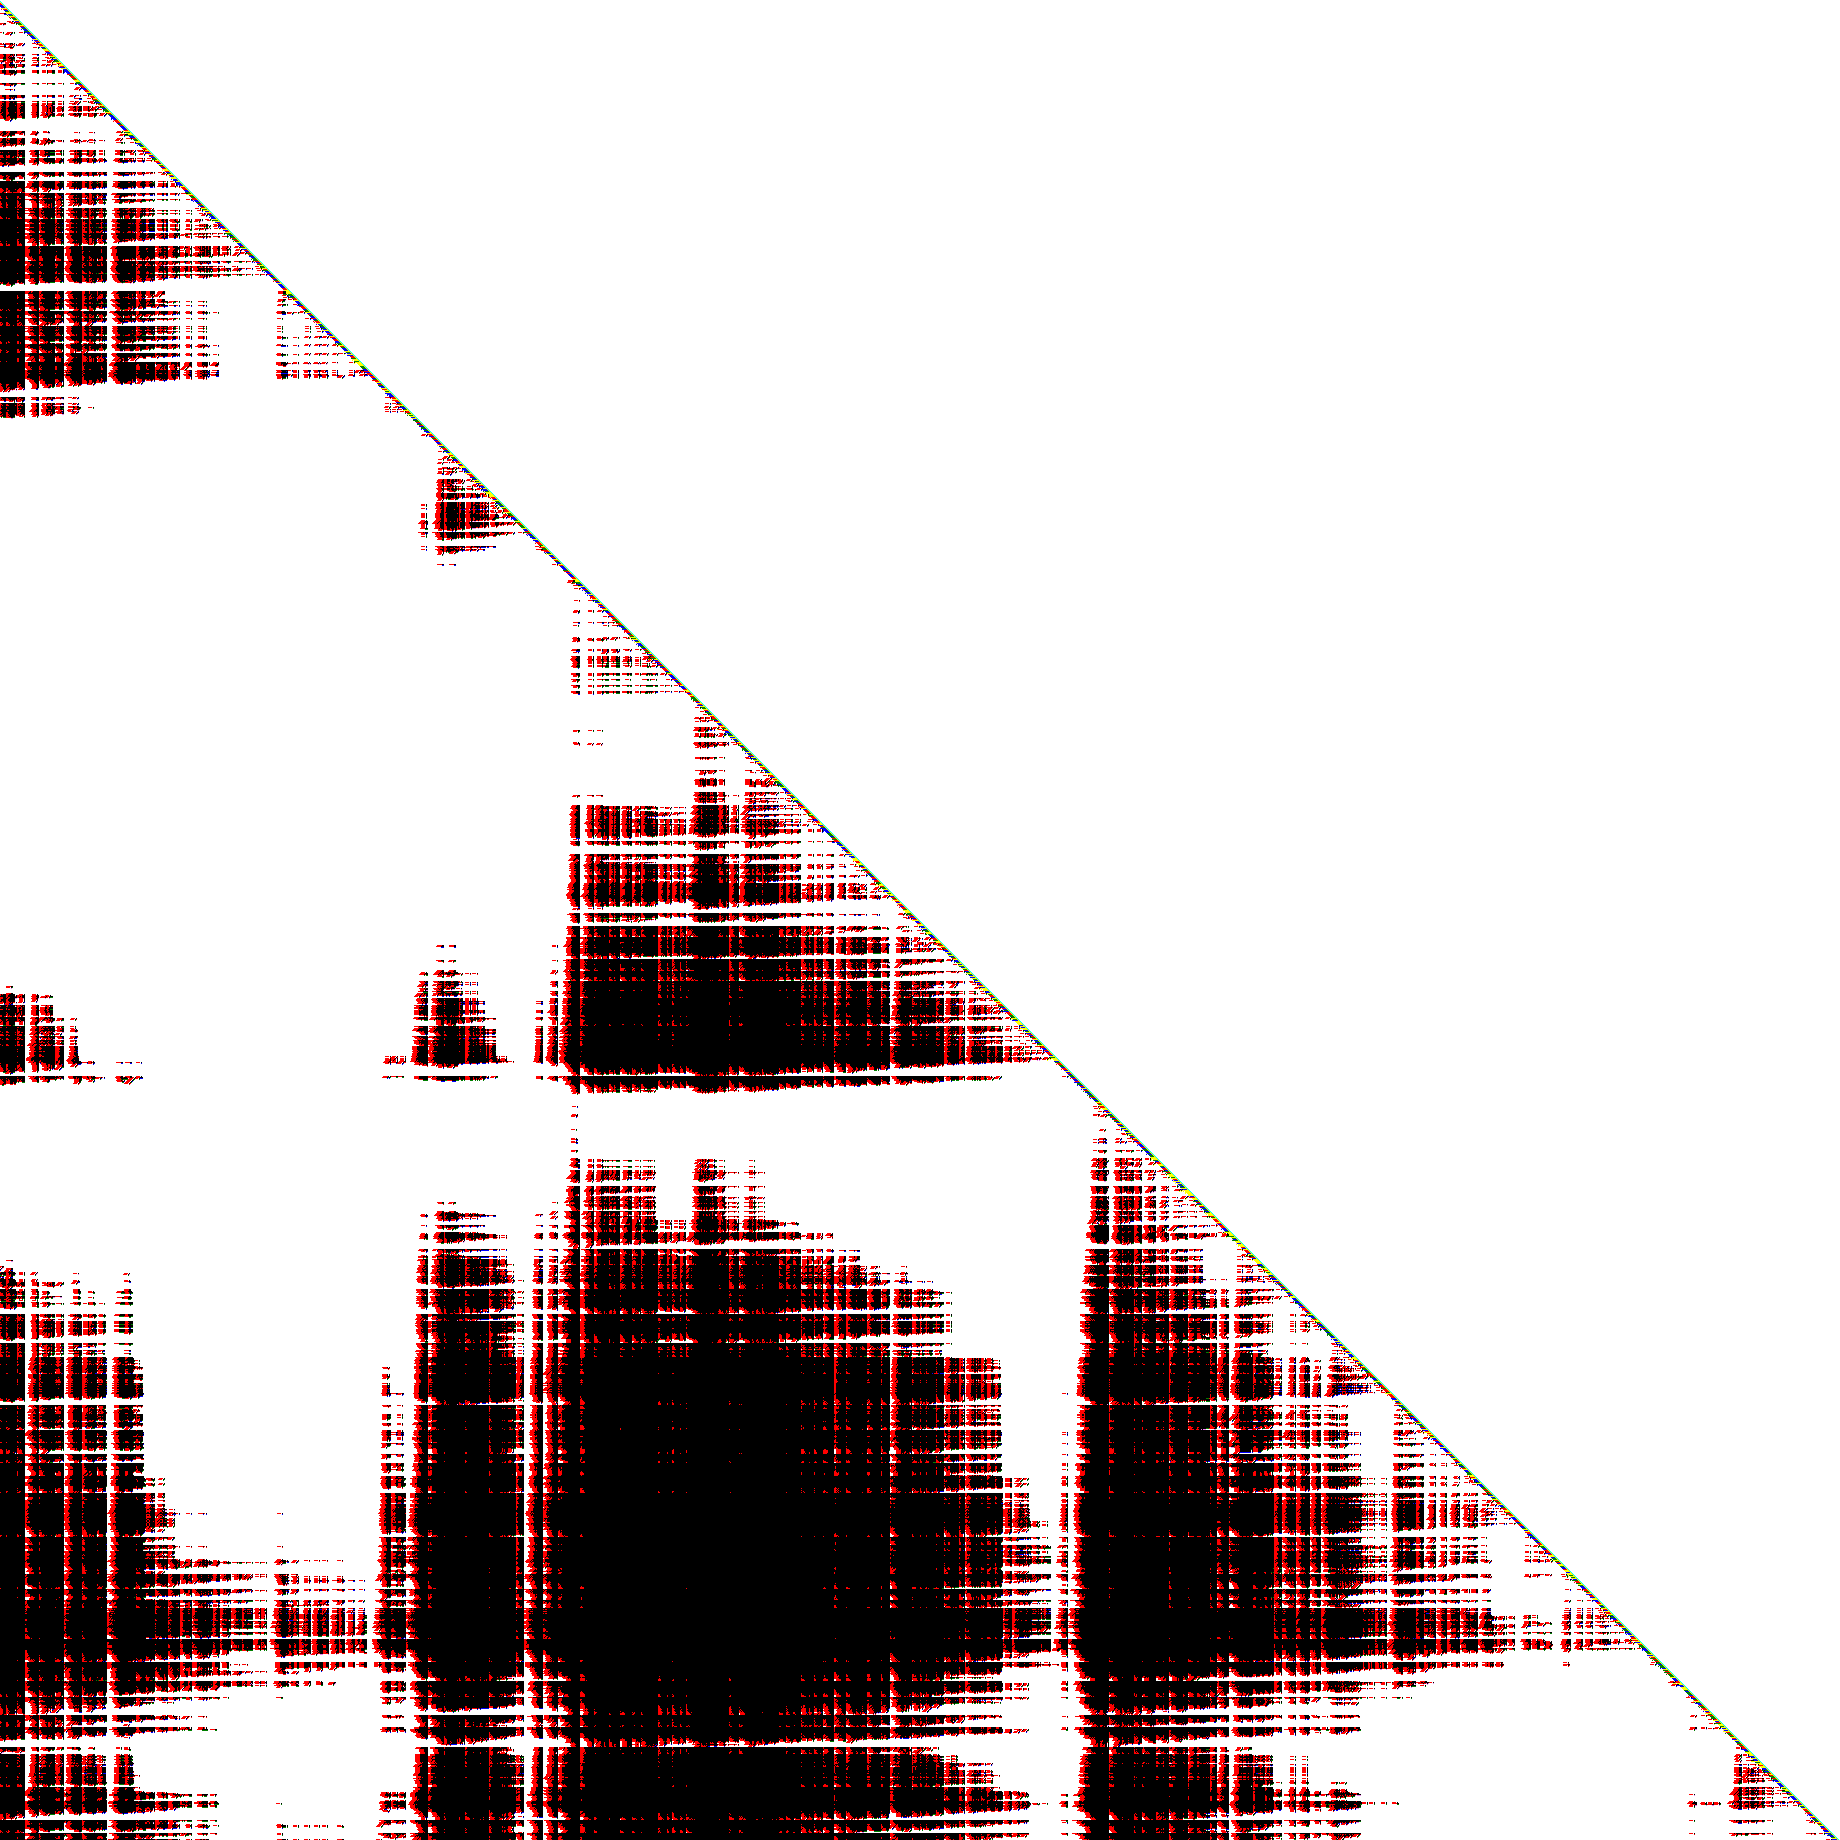
\includegraphics[height=5.4cm]{pictures/colored.png}
    \end{center}
  \end{tabular}
\end{frame}
      
\begin{frame}[fragile]
\transwipe[direction=90]
\frametitle{Задачи}
\begin{itemize}
\item Обработка (классификация, кластеризация и т.д.) изображений, представляющих информацию о вторичной структуре
\item Обработка (классификация, кластеризация и т.д.) векторных представлений данных о вторичной структуре
\item Подробное описание задач: \url{https://goo.gl/A2xyae}
\item ``Направления развития'': курсовая, диплом, публикации
\end{itemize}
\end{frame}

\begin{frame}
  \transwipe[direction=90]
  \frametitle{Требования к знаниям и навыкам}
  \begin{itemize}
    \item Методы и алгоритмы обработки данных, статистические методы, машинное обучение, обработка изображений
    \item Умение читать и понимать научные статьи
    \item Умение читать и понимать чужой код    
  \end{itemize}
\end{frame}


\begin{frame}[plain,c]
 \transwipe[direction=90]
 \begin{center}
  \Huge Синтаксический анализ графов на основе матричных операций
 \end{center}
\end{frame}

\begin{frame}[fragile]
\transwipe[direction=90]
\frametitle{Задачи}
\begin{itemize}
\item Цель: изучение возможностей построения эффективных алгоритмов синтаксического анализа графов
\item Задачи
\begin{itemize}
\item Исследование алгоритма синтаксического анализа линейного входа, основанного на матричных операциях, позволяющего повысить эффективность использования параллельных вычислений
\item Получение оценки сложности алгоритма синтаксического анализа графов в случае использования разреженных матриц для представления данных
\item Исследование возможности использовать алгоритма приближённого алгоритма перемножения матриц для приближённого синтаксического анализа графов
\item Оптимизация синтаксического анализа для DAG-ов и ``почти DAG-ов''
\end{itemize}
\item Подробное описание задач: \url{https://goo.gl/MB18nX}
\item ``Направления развития'': курсовая, диплом, публикации
\end{itemize}
\end{frame}

\begin{frame}
  \transwipe[direction=90]
  \frametitle{Требования к знаниям и навыкам}
  \begin{itemize}
    \item Теоретическая подготовка в области алгоритмов и анализе сложности, основы (линейной) алгебры
    \item Умение читать и понимать научные статьи
    \item Умение читать и понимать чужой код    
    \item Умение писать научные статьи/отчёты
    \item Знакомство с функциональным программированием (F\#, OCaml, Haskell и т.д.)
    \item Навыки работы с Git/GitHub
  \end{itemize}
\end{frame}


\begin{frame}[plain,c]
 \transwipe[direction=90]
 \begin{center}
  \Huge Парсер-комбинаторы для запросов к графовой базе данных
 \end{center}
\end{frame}

\begin{frame}[fragile]
\transwipe[direction=90]
\frametitle{Задачи}
\begin{itemize}
\item Цель: использование парсер-комбинаторов для запросов к графовым базам данных
\item Задачи
\begin{itemize}
\item Интеграция библиотеки парсер-комбинаторов на Scala с графовой базой данных Neo4J
\item Подготовка данных и проведение экспериментального исследования полученного решения
\end{itemize}
\item Подробное описание задач: \url{https://goo.gl/EaYKvY}
\item ``Направления развития'': курсовая, публикации
\end{itemize}
\end{frame}

\begin{frame}
  \transwipe[direction=90]
  \frametitle{Требования к знаниям и навыкам}
  \begin{itemize}
    \item Знакомство с языком программирования Scala
    \item Умение читать и понимать чужой код
    \item Базовые знания в области формальных языков, синтаксичского анализа, теории графов
    \item Навыки работы с Git/GitHub
  \end{itemize}
\end{frame}

            
\begin{frame}
\transwipe[direction=90]
\frametitle{Контакты}
\begin{itemize}
  \item Почта: \url{rsdpisuy@gmail.com}
  \item Исходный код YaccConstructor: \url{https://github.com/YaccConstructor}
\end{itemize}
\end{frame}
\end{document}
